\documentclass[a4paper,11pt]{article}

\usepackage[utf8]{inputenc}
\usepackage[swedish]{babel}
\usepackage[top=1in,bottom=1in,left=1in,right=1in,headsep=.5in]{geometry}
\usepackage{hyperref}
\usepackage{graphicx}

\usepackage{array}
\newcolumntype{L}[1]{>{\raggedright\let\newline\\\arraybackslash\hspace{0pt}}m{#1}}
\newcolumntype{C}[1]{>{\centering\let\newline\\\arraybackslash\hspace{0pt}}m{#1}}
\newcolumntype{R}[1]{>{\raggedleft\let\newline\\\arraybackslash\hspace{0pt}}m{#1}}

\usepackage[yyyymmdd,hhmmss]{datetime}
\renewcommand{\dateseparator}{-}

\usepackage{mathptmx}    %Times Roman font
\usepackage{helvet}    %Helvetica, served as a model for arial
\usepackage{anyfontsize}

\usepackage[tocgraduated]{tocstyle}
\usetocstyle{allwithdot}

\usepackage[titletoc,title]{appendix}

\usepackage{fancyhdr}
\fancypagestyle{intro}{
    \fancyhf{}
    \fancyhead[C]{\LIPSprojekttitel}
    \fancyhead[R]{\today} 
    \fancyfoot[L]{\LIPSkursnamn \\ \LIPSdokumenttyp}
    \fancyfoot[C]{\phantom{text}\roman{page}}
    \fancyfoot[R]{\LIPSprojektgrupp \\ \LIPSgruppepost} 
    \renewcommand{\headrulewidth}{0.4pt}
    \renewcommand{\footrulewidth}{0.4pt}}
\fancypagestyle{content}{
    \fancyhf{}
    \fancyhead[C]{\LIPSprojekttitel}
    \fancyhead[R]{\today} 
    \fancyfoot[L]{\LIPSkursnamn \\ \LIPSdokumenttyp}
    \fancyfoot[C]{\phantom{text}\thepage}
    \fancyfoot[R]{\LIPSprojektgrupp \\ \LIPSgruppepost} 
    \renewcommand{\headrulewidth}{0.4pt}
    \renewcommand{\footrulewidth}{0.4pt}}

\usepackage{titlesec}
\titleformat{\section}
    {\normalfont\sffamily\Large\bfseries}
    {\thesection}{1em}{}
\titleformat{\subsection}
    {\normalfont\sffamily\large\bfseries}
    {\thesubsection}{1em}{}
\titleformat{\subsubsection}
    {\normalfont\sffamily\bfseries}
    {\thesubsubsection}{1em}{}

\newcommand{\LIPSartaltermin}{2016/HT}
\newcommand{\LIPSkursnamn}{TSEA29}
\newcommand{\LIPSprojekttitel}{Kartrobot}
\newcommand{\LIPSprojektgrupp}{Grupp 1}
\newcommand{\LIPSgruppepost}{\href{mailto:kmm_2016_grupp1@liuonline.onmicrosoft.com}{{\small kmm\_2016\_grupp1@liuonline.onmicrosoft.com}}}
\newcommand{\LIPSgrupphemsida}{}
\newcommand{\LIPSkund}{ISY, Linköpings universitet, 581\,83 Linköping}
\newcommand{\LIPSkundkontakt}{Mattias Krysander, 013-282198, matkr@isy.liu.se}
\newcommand{\LIPSkursansvarig}{Tomas Svensson, 013-281368, Tomas.Svensson@liu.se}
\newcommand{\LIPShandledare}{}
\newcommand{\LIPSdokumenttyp}{Projektplan}
\newcommand{\LIPSredaktor}{Felix Härnström}
\newcommand{\LIPSversion}{0.1}
\newcommand{\LIPSgranskare}{}
\newcommand{\LIPSgranskatdatum}{}
\newcommand{\LIPSgodkannare}{}
\newcommand{\LIPSgodkantdatum}{}

\newcommand{\LIPStitelsida}{
\vspace*{200pt}
\renewcommand{\familydefault}{\sfdefault}	%Sans-serif
\normalfont
\begin{center}
{\fontsize{18}{22}\selectfont \textbf{\MakeUppercase{\LIPSdokumenttyp}}}
\end{center}
\begin{center}
{\fontsize{12}{14}\selectfont \LIPSredaktor \\[8pt] Version \LIPSversion}
\end{center}
\vspace*{220pt}
\begin{center}
{\fontsize{12}{14}\selectfont Status}
\end{center}
\begin{center}
\setlength\extrarowheight{2pt}
\begin{tabular}{| L{100pt} | L{100pt} | L{100pt} |}
\hline 
Granskad & \LIPSgranskare & \LIPSgranskatdatum \\
\hline 
Godkänd & \LIPSgodkannare & \LIPSgodkantdatum \\ 
\hline 
\end{tabular} 
\end{center}
\renewcommand{\familydefault}{\rmdefault}	%Back to serifs
\normalfont
}


\newenvironment{LIPSprojektidentitet}{%
\vspace*{200pt}
\renewcommand{\familydefault}{\sfdefault}	%Sans-serif
\normalfont
\begin{center}
{\fontsize{16}{19}\selectfont \textbf{PROJEKTIDENTITET}}
\end{center}
\renewcommand{\familydefault}{\rmdefault}	%Back to serifs
\normalfont
\begin{center}
\LIPSartaltermin, \LIPSprojektgrupp \\ Linköpings tekniska högskola, ISY
\end{center}
\renewcommand{\familydefault}{\sfdefault}	%Sans-serif
\normalfont
\vspace*{10pt}
\begin{center}
\setlength\extrarowheight{2pt}
\begin{tabular}{| L{100pt} | L{150pt} | L{150pt} |}
\hline
\textbf{Namn} & \textbf{Ansvar} & \textbf{E-post} \\
}%
{%
\hline
\end{tabular} 
\end{center}
\renewcommand{\familydefault}{\rmdefault}	%Back to serifs
\normalfont
\begin{center}
\textbf{E-postlista för hela gruppen:} \LIPSgruppepost \\
\textbf{Hemsida:} \LIPSgrupphemsida \\
\vspace*{15pt}
\textbf{Kund:} \LIPSkund \\
\textbf{Kontaktperson hos kund:} \LIPSkundkontakt \\
\vspace*{15pt}
\textbf{Kursansvarig:} \LIPSkursansvarig \\
\textbf{Handledare:} \LIPShandledare \\
\end{center}
}
\newcommand{\LIPSgruppmedlem}[3]{\hline {#1} & {#2} & \href{mailto:{#3}}{{#3}} \\}

\newenvironment{LIPSdokumenthistorik}{%
\vspace*{100pt}
\renewcommand{\familydefault}{\sfdefault}	%Sans-serif
\normalfont
\begin{center}
{\fontsize{14}{17}\selectfont \textbf{Dokumenthistorik}}
\end{center}
\begin{center}
\setlength\extrarowheight{2pt}
\begin{tabular}{| L{50pt} | L{60pt} | L{150pt} | L{60pt} | L{55pt} |}
\hline
\textbf{Version} & \textbf{Datum} & \textbf{Utförda förändringar} & \textbf{Utförda av} & \textbf{Granskad} \\
}%
{%
\hline
\end{tabular} 
\end{center}
\renewcommand{\familydefault}{\rmdefault}	%Back to serifs
\normalfont
}
\newcommand{\LIPSversionsinfo}[5]{\hline {#1} & {#2} & {#3} & {#4} & {#5} \\}

\newcounter{LIPSkravnummer}
\newcounter{LIPSunderkravnummer}[LIPSkravnummer]
\newenvironment{LIPSkravlista}{%
\renewcommand{\familydefault}{\sfdefault}	%Sans-serif
\normalfont
 \setlength\extrarowheight{2pt}
  \begin{tabular}{| L{30pt } | L{60pt} | L{250pt} | L{50pt} |}
    }%
  {%
    \hline
  \end{tabular}
\renewcommand{\familydefault}{\rmdefault}	%Back to serifs
\normalfont
}
\newcommand{\LIPSkrav}[3]{\hline\stepcounter{LIPSkravnummer}\textbf{\arabic{LIPSkravnummer}} & \textbf{{#1}} & {#2} & \textbf{{#3}} \\}

\newcommand{\LIPSkravDemo}[3]{\hline\textbf{X} & \textbf{{#1}} & {#2} & \textbf{{#3}} \\}

\newcommand{\LIPSunderkrav}[3]{\hline\stepcounter{LIPSunderkravnummer}\textbf{\arabic{LIPSkravnummer}\Alph{LIPSunderkravnummer}} & \textbf{{#1}} & {#2} & \textbf{{#3}} \\}


\newenvironment{LIPSleveranslista}{
\renewcommand{\familydefault}{\sfdefault}	%Sans-serif
\normalfont
	\setlength\extrarowheight{2pt}
	\begin{tabular}{| L{25mm} | L{25mm} | L{55mm} | L{25mm} | L{5mm} |} 
	}
	{
		\hline
	\end{tabular}
\renewcommand{\familydefault}{\rmdefault}	%Back to serifs
\normalfont
}
\newcommand{\LIPSleverans}[4]{ \hline\stepcounter{LIPSkravnummer}\textbf{Krav nr \arabic{LIPSkravnummer}}&\textbf{{#1}}&{#2}&\textbf{{#3}}&\textbf{{#4}}\\}


\newenvironment{LIPSdokumentlista}{%
	\renewcommand{\familydefault}{\sfdefault}	%Sans-serif
	\normalfont
	\setlength\extrarowheight{2pt}
	\begin{tabular}{| L{40mm} | L{13mm} | L{50mm} | L{19mm} | L{14mm} |} 
		
		\hline
		\textbf{Dokument} & \textbf{Språk} & \textbf{Syfte/Innehåll} & \textbf{Målgrupp} & \textbf{Format} \\
	}%
	{%
		\hline
	\end{tabular}
	\renewcommand{\familydefault}{\rmdefault}	%Back to serifs
	\normalfont
}
\newcommand{\LIPSdokument}[5]{\hline {#1} & {#2} & {#3} & {#4} & {#5}\\}

\begin{document}
\pagestyle{intro}
\LIPStitelsida
\clearpage
\begin{LIPSprojektidentitet}
    \LIPSgruppmedlem{Hannes Haglund}{Designansvarig mjukvara (MV)}{hanha265@student.liu.se}
    \LIPSgruppmedlem{Felix Härnström}{Projektledare (PL)}{felha423@student.liu.se}
    \LIPSgruppmedlem{Jani Jokinen}{Leveransansvarig (LEV)}{janjo273@student.liu.se}
    \LIPSgruppmedlem{Silas Lenz}{Testansvarig (TST)}{sille914@student.liu.se}
    \LIPSgruppmedlem{Daniel Månsson}{Designansvarig hårdvara (HV)}{danma344@student.liu.se}
    \LIPSgruppmedlem{Emil Norberg}{Dokumentansvarig (DOK)}{emino969@student.liu.se}
\end{LIPSprojektidentitet}
\clearpage
\renewcommand{\familydefault}{\sfdefault}	%Sans-serif
\normalfont
\tableofcontents
\renewcommand{\familydefault}{\rmdefault}	%Back to serifs
\normalfont
\clearpage
\begin{LIPSdokumenthistorik}
    \LIPSversionsinfo{0.1}{2016-09-07}{Första utkastet}{}{}
\end{LIPSdokumenthistorik}
\clearpage
\setcounter{page}{1}
\pagestyle{content}
\section{Beställare}
Beställare är Mattias Kryssander från ISY vid Linköpings universitet.

\section{Översiktlig beskrivning av projektet}
\subsection{Syfte och mål}
Projektet mål är att utefter givet projektdirektiv och med beställaren överenskommen kravspecifikation utveckla en robot som kan genomsöka och kartlägga ett enkelt rum. Utöver roboten ska en medföljande PC-mjukvara levereras som kan styra roboten och visa realtidsdata såsom diagnostik och kartan över rummet.

\subsection{Leveranser}
\begin{flushleft}
\begin{LIPSleveransplan}
    \LIPSplaneradleverans{Projektplan, tidsplan, och systemskiss}{PL}{Första version av projektplan, tidsplan, och systemskiss}{2016-09-22}
    \LIPSplaneradleverans{Projektplan, tidsplan, och systemskiss}{PL}{Slutgiltig version av projektplan, tidsplan, och systemskiss}{2016-09-22}
    \LIPSplaneradleverans{Tidrapport}{PL}{Tidrapport 1.}{2016-10-31}
    \LIPSplaneradleverans{Designspecifikation}{PL}{Första version av designspecifikationen.}{2016-11-01}
    \LIPSplaneradleverans{Designspecifikation}{PL}{Slutgiltig version av designspecifikation.}{2016-11-04}
    \LIPSplaneradleverans{Tidrapport}{PL}{Tidrapport 2.}{2016-11-7}
    \LIPSplaneradleverans{Tidrapport}{PL}{Tidrapport 3.}{2016-11-14}
    \LIPSplaneradleverans{Tidrapport}{PL}{Tidrapport 4.}{2016-11-21}
    \LIPSplaneradleverans{Tidrapport}{PL}{Tidrapport 5.}{2016-11-28}
    \LIPSplaneradleverans{Tidrapport}{PL}{Tidrapport 6.}{2016-12-5}
    \LIPSplaneradleverans{Tidrapport}{PL}{Tidrapport 7.}{2016-12-12}
    \LIPSplaneradleverans{Teknisk dokumentation och användarhandledning}{PL}{Teknisk dokumentation och användarhandledning ska vara inlämnad.}{3 arbetsdagar före redovisning.}
    \LIPSplaneradleverans{Verifiering av kraven (BP5).}{PL}{Tillsammans med beställaren fattas beslut huruvida projektet har nått målet.}{Senast dagen innan redovisning.}
    \LIPSplaneradleverans{Tidrapport}{PL}{Tidrapport 8.}{2016-12-19}
    \LIPSplaneradleverans{Slutpresentation}{PL}{Muntlig presentation av projektet.}{2016-12-19}
    \LIPSplaneradleverans{Tävlingsdeltagande}{PL}{Tävla mot andra robotar som har byggts i kursen.}{2016-12-20}
    \LIPSplaneradleverans{Efterstudie}{PL}{Efterstudie ska lämnas till beställaren.}{2016-12-21}
    \LIPSplaneradleverans{Källkod}{PL}{Källkod ska lämnas till beställaren.}{2016-12-21}
    \LIPSplaneradleverans{Utrustning}{PL}{All utrustning ska återlämnas.}{2016-12-22}
\end{LIPSleveransplan}
\end{flushleft}

\subsection{Begränsningar}
Produkten är vid slutleverans begränsad till de krav som är formulerade i den senaste versionen av kravspecifikationen. 

\section{Fasplan}

\section{Organisationsplan för hela projektet}
Projektgruppen och utomstående resurser är organiserade såsom beskrivet i figur \ref{fig:org}. Utöver denna grova organisationsplan kan projektgruppen bilda interna arbetsgrupper vid behov.

\begin{figure}[h!]
\centering
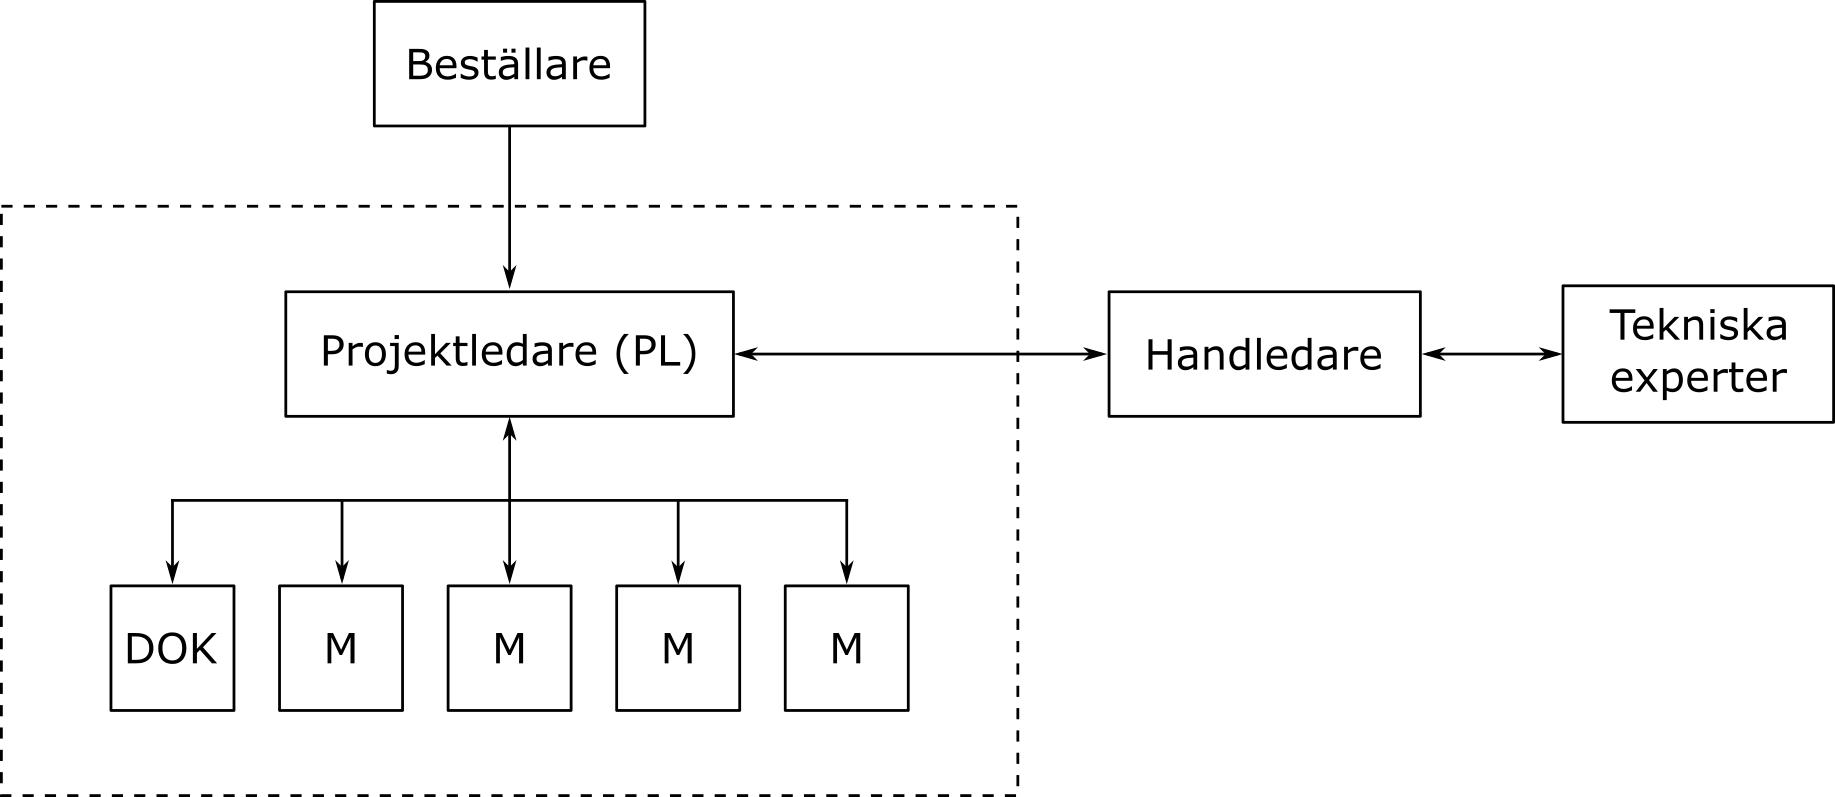
\includegraphics[scale=1]{organisation.png}
\caption{Översiktlig projektorganisation.}
\label{fig:org}
\end{figure}

\section{Dokumentplan}

\section{Utvecklingsmetodik}

\section{Utbildningsplan}

\subsection{Egen utbildning}

\subsection{Kunden utbildning}

\section{Rapporteringsplan}

\section{Mötesplan}

\section{Resursplan}
\subsection{Personer}
\subsection{Material}

\subsection{Lokaler}

\subsection{Ekonomi}

\section{Milstolpar och beslutspunkter}
\subsection{Milstolpar}
\subsection{Beslutspunkter}

\section{Aktiviteter}

\section{Tidplan}

\section{Förändringsplan}

\section{Kvalitetsplan}

\subsection{Granskningar}

\subsection{Testplan}

\section{Riskanalys}

\section{Prioriteringar}

\section{Projektavslut}

\begin{appendices}
\end{appendices}
\end{document}
